\section{Понятия о методах спуска}

\[  
  A \overline{\vec{x}} = b \iff F(\overline{\vec{x}}) = \min_{\vec{x}}
  F(\vec{x})
\]

$A$ --- симметричная, положительно определенная.

\begin{align*}
  F(x) &= \frac 12 \sum_{i = 1}^n \sum_{j = 1}^n a_{ij} x_i x_j - \sum_{i = 1}^n b_i x_i =\\ 
       &= \frac 12 (A\vec{x}, \vec{x}) - (\vec{b}, \vec{x})
\end{align*}

Для положительно определенной квадратичной формы необходимое условие минимумма
будет и достаточным.
\[
  \frac{\partial F}{\partial x_k} = 0,\ k = 1, \dotsc, n
\]

\begin{gather*}
  \frac{\partial F}{\partial x_k} = \frac 12 \sum_{j = 1}^n a_{kj}x_j + \frac 12
  \sum_{i = 1}^n a_{ki}x_i - b_k = 0,\ k = 1,\dotsc, n \\
  \sum_{j = 1}^n a_{kj} x_j - b_k = 0,\ \sum_{j = 1}^n a_{kj}x_j = b_k,\ k = 1,
  \dotsc, n
\end{gather*}

\begin{align*}
  \vec{x}^0, \vec{p}^0: &F(\vec{x}^0 + \alpha \vec{p}^0) \underset{<}{\alpha \to
                          0} F(\vec{x}^0)\\
                        &F(\vec{x}^0 + \alpha^0 \vec{p}^0) < F(\vec{x}^0)
                        &\vec{x}^1 = \vec{x}^0 + \alpha_0 \vec{p}^0
\end{align*}

\subsection{Направления спуска}
\begin{gather*}
  \frac{F(\vec{x}^0 + \alpha \vec{p}^0) - F(x^0)}{\frac{d}{d\alpha} F(\vec{x}^0
    + \alpha \vec{p}^0)} \underset{<}{\alpha \to 0} 0 \\
  \sum_{i = 1}^n \frac{\partial F}{\partial x_i} |_{\vec{x}^0} P_i < 0\\
  \nabla F |_{\vec{x}^0} \cdot \vec{p}^0 < 0
\end{gather*}

Выбор шага: $F(\vec x^0 + \alpha^0 \vec p^0) = \min\limits_\alpha F(\vec x^0 + \alpha p^0)$

\begin{gather*}
F(x^0 + \alpha \vec p^0) = \frac12 \left[ \text{хз что тут было}\right] \\
  = \frac12 (A\vec x^0, \vec x^0) + \frac{\vec\alpha}{2} (A \vec p^0, \vec x^0) +
  \frac{\alpha^2}2(A\vec x^0, \vec p^0) - (\vec b, \vec x^0) - \alpha(\vec b, \vec p^0) = \\
  = \frac{\alpha^2}{2} (A \vec p^0, \vec p^0) + \alpha (A \vec x^0, \vec p^0) -
  \alpha(\vec b, \vec p^0) + \frac12 (A\vec x^0, \vec x^0) - (\vec b, \vec x^0) \\
  = \frac{\alpha^2}{2} (A \vec p^0, \vec p^0) + \alpha (A \vec x^0, p^0) + \frac12(A\vec x^0, \vec x^0) - (\vec b, \vec x^0)
\end{gather*}
\begin{align*}
  \frac{dF(x^0 + \alpha {\vec p}^0}{d\alpha} = 0, \quad \alpha(A\vec p^0, \vec p^0) + (A \vec x^0 - \vec b, \vec p^0) = 0 \\
                      \alpha = \alpha^0 = -\frac{(A \vec x^0 - \vec b, \vec p^0)}{(A\vec p^0, \vec p^0)} = -\frac{(\vec g^0, \vec p^0)}{(A\vec p^0, \vec p^0)}
\end{align*}


\subsection{Покоординатный спуск}
\begin{gather*}
  \vec{x}_k =
  \begin{pmatrix}
    x_1^k\\
    x_2^k\\
    \vdots\\
    x_n^k
  \end{pmatrix} \\
  \min_{x_1} F(x_1, x_2^k, x_3^k, \dotsc, x_n^k) = F(x_1^{k + 1}, x_2^k,
  \dotsc, x_n^k) \\
  \min_{x_2} F(x_1^{k + 1}, x_2, x_3^k, \dotsc, x_n^k) = F(x_1^{k + 1}, x_2^{k +
    1}, \dotsc, x_n^k)\\
  \vdots
  \min_{x_i} F(x_1^{k + 1}, x_2^{k + 1}, \dotsc, x_i, x_{i + 1}^k, \dotsc,
  x_n^k) = F(x_1^{k + 1}, \dotsc, x_i^{k + 1}, x_{i + 1}^k, \dotsc, x_n^k) \\
  \frac{\partial F}{\partial x_i}= 0\\
  \sum_{j = 1}^{i - 1} a_{ij}x_j^{k + 1} + a_{ii}x_i + \sum_{j = i + 1}^n
  a_{ij}x_j^k = 0 \\
  x_i = - \sum_{j = 1}^{i - 1} \frac{a_{ij}}{a_{ii}} x_j^{k = 1} - \sum_{j = i +
  1}^n \frac{a_{ij}}{a_{ii}}x_j^k 
\end{gather*}

\subsection{Метод наискорейшего спуска}
\begin{figure}[h]
  \centering
  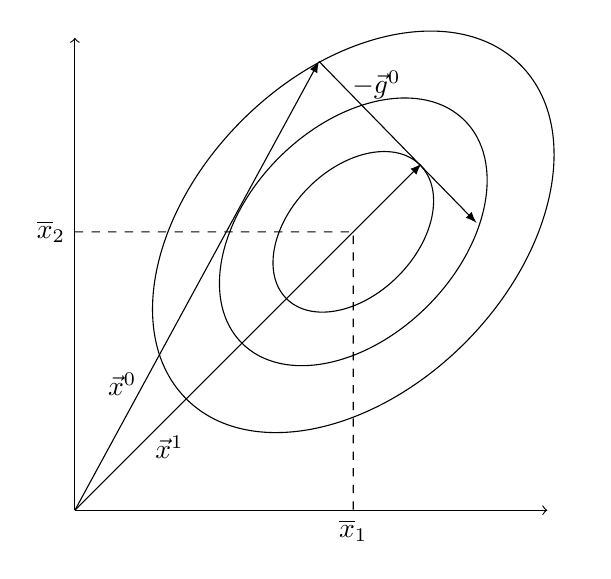
\begin{tikzpicture}
 % \draw (0,0) circle(.1em);
  \draw[rotate=45] (5, 0) ellipse (3 and 2);
  \draw[rotate=45] (5, 0) ellipse (2 and 1.33333);
  \draw[rotate=45] (5, 0) ellipse (1.2 and .8);

  %% оси
  \draw[->] (0, 0) -- (0, 6);
  \draw[->] (0, 0) -- (6, 0);
  \node[left] at (0, 3.5355) {$\overline x_2$};
  \draw[dashed] (0, 3.5355) -- (45:5) -- (3.5355, 0);
  \node[below] at (3.5355, 0) {$\overline x_1$};

  \draw[-latex] (0, 0) -- (3.1,5.7);
  \node at (.6,  1.6) {$\vec x^0$};
  \draw[-latex] (0, 0) -- (4.4, 4.4);
  \node[above right] at (3.4, 5.1) {$-\vec g^0$};
  \node at (1.2, .8) {$\vec x^1$};
  \draw[-latex] (3.1, 5.7) -- (5.1, 3.65);
\end{tikzpicture}
  \caption{Двумерный случай, эллипсы — изолинии}
\end{figure}
\begin{gather*}
  \vec{p}^k = -\vec{g}^k \\
  \alpha^k = \frac{(\vec{g}^k, \vec{g}^k)}{(A \vec{g}^k, \vec{g}^k)} \\
  \vec{x}^{k + 1} = \vec{x}^k - \alpha^k \vec{g}^k \\
  \|\vec{x}^k - \overline{\vec{x}}\| \leq
  \sqrt{\frac{\lambda_{max}}{\lambda_{min}}} (\frac{\lambda_{max} -
    \lambda_{min}}{\lambda_{max} + \lambda_{min}})^k \|\vec{x}^0
  -\overline{\vec{x}}\| \text{ --- априорная оценка сходимости}\\
\end{gather*}

\subsection{Методы сопряженных направлений}
\begin{gather*}
   \vec{p}^0, \vec{x}^1, \dotsc, \vec{x}^{n - 1} : (A\vec{p}^i, \vec{p}^j) = 0,\
   i \neq j
\end{gather*}

\subsection{Метод сопряжённых градиентов}
\begin{gather*}
  \vec{x}^0,\ \vec{p}^0 = -\vec{g}^0,\ \alpha^0 = \frac{(\vec{g}^0,
    \vec{g}^0)}{(A\vec{g}^0, \vec{g}^0)},\ \vec{x}^1 = \vec{x}^0 - \alpha_0
  \vec{g}^0 \\ 
  \vec{p}^1 = -\vec{g}^1 + \beta^0 \vec{p}^0,\ \beta^0 =
  \frac{(A\vec{p}^0, \vec{p}^0)}{(A\vec{p}^0, \vec{p}^0)},\ \alpha_1 =
  \frac{(\vec{g}^1, \vec{po}^1)}{(A\vec{p}^1, \vec{p}^1)},\ x^2 = \vec{x}^1 + \alpha^1 \vec{p}^1
\end{gather*}
